\documentclass[tikz, margin=1mm]{standalone}
\usepackage[utf8]{inputenc}
\usepackage{tikz}
\renewcommand{\familydefault}{\sfdefault}
% \usepackage{sansmath}
% \sansmath

% Convert pdf to pngs using
% pdftoppm -png -r 450 acoustic_bsdf.pdf acoustic_bsdf

\usetikzlibrary{
	math,
	% decorations.pathreplacing,
	% decorations.pathmorphing,
	% calligraphy,
	% calc,
	% positioning,
	% shapes,
	% fit,
	% backgrounds
}
\tikzstyle{arrow} = [very thick,->,>=stealth]






\begin{document}


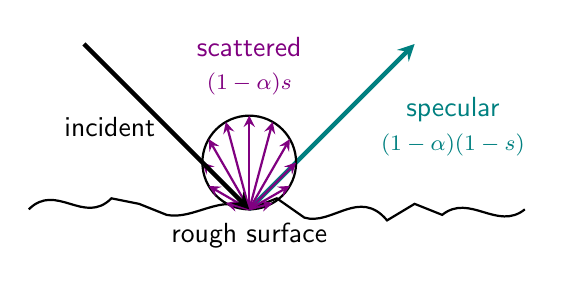
\begin{tikzpicture}[scale=0.7]
	\draw[thick] (-4, 0) .. controls (-3.5, 0.5) and (-3, -0.3) .. (-2.5, 0.2)
	-- (-2, 0.1) -- (-1.5, -0.1)
	.. controls (-1, -0.2) and (-0.5, 0.3) .. (0, -0.)
	-- (0.5, 0.2) -- (1, -0.15)
	.. controls (1.5, -0.3) and (2, 0.4) .. (2.5, -0.2)
	-- (3, 0.1) -- (3.5, -0.1)
	.. controls (4, 0.3) and (4.5, -0.4) .. (5, 0);
	\node[below=-3mm] at (0, -0.5) {rough surface};

	\draw[arrow, teal, ultra thick] (0,0) -- (3,3);


	% Scattered rays
	% circle that shows lambert law
	\draw[thick] (0, 0.85) circle (0.85);

	\foreach \index in {1,2,3,4,5,6,7,8,9,10,11} {
			\pgfmathsetmacro{\angle}{180*\index/12}
			\pgfmathsetmacro{\length}{1.7*sin(\angle)+(rnd-0.5)*0.}
			\draw[arrow, thick, violet] (0, 0) -- ({\length*cos(\angle)}, {\length*sin(\angle)});
		}

	% Incident ray
	\draw[arrow, ultra thick] (-3, 3) -- (0, 0) node[midway, left] {incident};

	% labels
	\node[above, violet, align=center, opacity=1] at (0, 1.9) {scattered\\\footnotesize{$(1-\alpha) s$}};
	\node[right=0.5cm, teal,align=center, opacity=1] at (1.5, 1.5) {specular\\\footnotesize{$(1-\alpha) (1-s)$}};

\end{tikzpicture}


%% rendering plots of specular / scattering





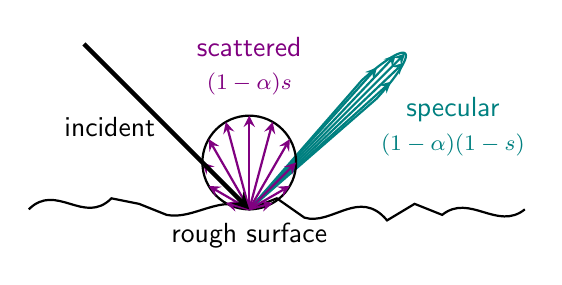
\begin{tikzpicture}[scale=0.7]
	\draw[thick] (-4, 0) .. controls (-3.5, 0.5) and (-3, -0.3) .. (-2.5, 0.2)
	-- (-2, 0.1) -- (-1.5, -0.1)
	.. controls (-1, -0.2) and (-0.5, 0.3) .. (0, -0.)
	-- (0.5, 0.2) -- (1, -0.15)
	.. controls (1.5, -0.3) and (2, 0.4) .. (2.5, -0.2)
	-- (3, 0.1) -- (3.5, -0.1)
	.. controls (4, 0.3) and (4.5, -0.4) .. (5, 0);
	\node[below=-3mm] at (0, -0.5) {rough surface};

	\tikzmath{\width=10;}
	\foreach \index in {2,3.5,5,6.5,8} {
			\pgfmathsetmacro{\angle}{40+\index}
			\pgfmathsetmacro{\length}{4*cos((\angle-45)*\width)}
			\draw[arrow, thick, teal] (0, 0) -- ({\length*cos(\angle)}, {\length*sin(\angle)});
		}
	\draw[thick, teal] plot[] coordinates {
			({0}, {0})
			({4*cos((41.0-45)*\width)*cos(41.0)},   {4*cos((41.0-45)*\width)*sin(41.0)})
			({4*cos((41.1-45)*\width)*cos(41.1)},   {4*cos((41.1-45)*\width)*sin(41.1)})
			({4*cos((41.2-45)*\width)*cos(41.2)},   {4*cos((41.2-45)*\width)*sin(41.2)})
			({4*cos((41.3-45)*\width)*cos(41.3)},   {4*cos((41.3-45)*\width)*sin(41.3)})
			({4*cos((41.4-45)*\width)*cos(41.4)},   {4*cos((41.4-45)*\width)*sin(41.4)})
			({4*cos((41.5-45)*\width)*cos(41.5)},   {4*cos((41.5-45)*\width)*sin(41.5)})
			({4*cos((41.6-45)*\width)*cos(41.6)},   {4*cos((41.6-45)*\width)*sin(41.6)})
			({4*cos((41.7-45)*\width)*cos(41.7)},   {4*cos((41.7-45)*\width)*sin(41.7)})
			({4*cos((41.8-45)*\width)*cos(41.8)},   {4*cos((41.8-45)*\width)*sin(41.8)})
			({4*cos((41.9-45)*\width)*cos(41.9)},   {4*cos((41.9-45)*\width)*sin(41.9)})
			({4*cos((42.0-45)*\width)*cos(42.0)},   {4*cos((42.0-45)*\width)*sin(42.0)})
			({4*cos((42.1-45)*\width)*cos(42.1)},   {4*cos((42.1-45)*\width)*sin(42.1)})
			({4*cos((42.2-45)*\width)*cos(42.2)},   {4*cos((42.2-45)*\width)*sin(42.2)})
			({4*cos((42.3-45)*\width)*cos(42.3)},   {4*cos((42.3-45)*\width)*sin(42.3)})
			({4*cos((42.4-45)*\width)*cos(42.4)},   {4*cos((42.4-45)*\width)*sin(42.4)})
			({4*cos((42.5-45)*\width)*cos(42.5)},   {4*cos((42.5-45)*\width)*sin(42.5)})
			({4*cos((42.6-45)*\width)*cos(42.6)},   {4*cos((42.6-45)*\width)*sin(42.6)})
			({4*cos((42.7-45)*\width)*cos(42.7)},   {4*cos((42.7-45)*\width)*sin(42.7)})
			({4*cos((42.8-45)*\width)*cos(42.8)},   {4*cos((42.8-45)*\width)*sin(42.8)})
			({4*cos((42.9-45)*\width)*cos(42.9)},   {4*cos((42.9-45)*\width)*sin(42.9)})
			({4*cos((43.0-45)*\width)*cos(43.0)},   {4*cos((43.0-45)*\width)*sin(43.0)})
			({4*cos((43.1-45)*\width)*cos(43.1)},   {4*cos((43.1-45)*\width)*sin(43.1)})
			({4*cos((43.2-45)*\width)*cos(43.2)},   {4*cos((43.2-45)*\width)*sin(43.2)})
			({4*cos((43.3-45)*\width)*cos(43.3)},   {4*cos((43.3-45)*\width)*sin(43.3)})
			({4*cos((43.4-45)*\width)*cos(43.4)},   {4*cos((43.4-45)*\width)*sin(43.4)})
			({4*cos((43.5-45)*\width)*cos(43.5)},   {4*cos((43.5-45)*\width)*sin(43.5)})
			({4*cos((43.6-45)*\width)*cos(43.6)},   {4*cos((43.6-45)*\width)*sin(43.6)})
			({4*cos((43.7-45)*\width)*cos(43.7)},   {4*cos((43.7-45)*\width)*sin(43.7)})
			({4*cos((43.8-45)*\width)*cos(43.8)},   {4*cos((43.8-45)*\width)*sin(43.8)})
			({4*cos((43.9-45)*\width)*cos(43.9)},   {4*cos((43.9-45)*\width)*sin(43.9)})
			({4*cos((44.0-45)*\width)*cos(44.0)},   {4*cos((44.0-45)*\width)*sin(44.0)})
			({4*cos((44.1-45)*\width)*cos(44.1)},   {4*cos((44.1-45)*\width)*sin(44.1)})
			({4*cos((44.2-45)*\width)*cos(44.2)},   {4*cos((44.2-45)*\width)*sin(44.2)})
			({4*cos((44.3-45)*\width)*cos(44.3)},   {4*cos((44.3-45)*\width)*sin(44.3)})
			({4*cos((44.4-45)*\width)*cos(44.4)},   {4*cos((44.4-45)*\width)*sin(44.4)})
			({4*cos((44.5-45)*\width)*cos(44.5)},   {4*cos((44.5-45)*\width)*sin(44.5)})
			({4*cos((44.6-45)*\width)*cos(44.6)},   {4*cos((44.6-45)*\width)*sin(44.6)})
			({4*cos((44.7-45)*\width)*cos(44.7)},   {4*cos((44.7-45)*\width)*sin(44.7)})
			({4*cos((44.8-45)*\width)*cos(44.8)},   {4*cos((44.8-45)*\width)*sin(44.8)})
			({4*cos((44.9-45)*\width)*cos(44.9)},   {4*cos((44.9-45)*\width)*sin(44.9)})
			({4*cos((45.0-45)*\width)*cos(45.0)},   {4*cos((45.0-45)*\width)*sin(45.0)})
			({4*cos((45.1-45)*\width)*cos(45.1)},   {4*cos((45.1-45)*\width)*sin(45.1)})
			({4*cos((45.2-45)*\width)*cos(45.2)},   {4*cos((45.2-45)*\width)*sin(45.2)})
			({4*cos((45.3-45)*\width)*cos(45.3)},   {4*cos((45.3-45)*\width)*sin(45.3)})
			({4*cos((45.4-45)*\width)*cos(45.4)},   {4*cos((45.4-45)*\width)*sin(45.4)})
			({4*cos((45.5-45)*\width)*cos(45.5)},   {4*cos((45.5-45)*\width)*sin(45.5)})
			({4*cos((45.6-45)*\width)*cos(45.6)},   {4*cos((45.6-45)*\width)*sin(45.6)})
			({4*cos((45.7-45)*\width)*cos(45.7)},   {4*cos((45.7-45)*\width)*sin(45.7)})
			({4*cos((45.8-45)*\width)*cos(45.8)},   {4*cos((45.8-45)*\width)*sin(45.8)})
			({4*cos((45.9-45)*\width)*cos(45.9)},   {4*cos((45.9-45)*\width)*sin(45.9)})
			({4*cos((46.0-45)*\width)*cos(46.0)},   {4*cos((46.0-45)*\width)*sin(46.0)})
			({4*cos((46.1-45)*\width)*cos(46.1)},   {4*cos((46.1-45)*\width)*sin(46.1)})
			({4*cos((46.2-45)*\width)*cos(46.2)},   {4*cos((46.2-45)*\width)*sin(46.2)})
			({4*cos((46.3-45)*\width)*cos(46.3)},   {4*cos((46.3-45)*\width)*sin(46.3)})
			({4*cos((46.4-45)*\width)*cos(46.4)},   {4*cos((46.4-45)*\width)*sin(46.4)})
			({4*cos((46.5-45)*\width)*cos(46.5)},   {4*cos((46.5-45)*\width)*sin(46.5)})
			({4*cos((46.6-45)*\width)*cos(46.6)},   {4*cos((46.6-45)*\width)*sin(46.6)})
			({4*cos((46.7-45)*\width)*cos(46.7)},   {4*cos((46.7-45)*\width)*sin(46.7)})
			({4*cos((46.8-45)*\width)*cos(46.8)},   {4*cos((46.8-45)*\width)*sin(46.8)})
			({4*cos((46.9-45)*\width)*cos(46.9)},   {4*cos((46.9-45)*\width)*sin(46.9)})
			({4*cos((47.0-45)*\width)*cos(47.0)},   {4*cos((47.0-45)*\width)*sin(47.0)})
			({4*cos((47.1-45)*\width)*cos(47.1)},   {4*cos((47.1-45)*\width)*sin(47.1)})
			({4*cos((47.2-45)*\width)*cos(47.2)},   {4*cos((47.2-45)*\width)*sin(47.2)})
			({4*cos((47.3-45)*\width)*cos(47.3)},   {4*cos((47.3-45)*\width)*sin(47.3)})
			({4*cos((47.4-45)*\width)*cos(47.4)},   {4*cos((47.4-45)*\width)*sin(47.4)})
			({4*cos((47.5-45)*\width)*cos(47.5)},   {4*cos((47.5-45)*\width)*sin(47.5)})
			({4*cos((47.6-45)*\width)*cos(47.6)},   {4*cos((47.6-45)*\width)*sin(47.6)})
			({4*cos((47.7-45)*\width)*cos(47.7)},   {4*cos((47.7-45)*\width)*sin(47.7)})
			({4*cos((47.8-45)*\width)*cos(47.8)},   {4*cos((47.8-45)*\width)*sin(47.8)})
			({4*cos((47.9-45)*\width)*cos(47.9)},   {4*cos((47.9-45)*\width)*sin(47.9)})
			({4*cos((48.0-45)*\width)*cos(48.0)},   {4*cos((48.0-45)*\width)*sin(48.0)})
			({4*cos((48.1-45)*\width)*cos(48.1)},   {4*cos((48.1-45)*\width)*sin(48.1)})
			({4*cos((48.2-45)*\width)*cos(48.2)},   {4*cos((48.2-45)*\width)*sin(48.2)})
			({4*cos((48.3-45)*\width)*cos(48.3)},   {4*cos((48.3-45)*\width)*sin(48.3)})
			({4*cos((48.4-45)*\width)*cos(48.4)},   {4*cos((48.4-45)*\width)*sin(48.4)})
			({4*cos((48.5-45)*\width)*cos(48.5)},   {4*cos((48.5-45)*\width)*sin(48.5)})
			({4*cos((48.6-45)*\width)*cos(48.6)},   {4*cos((48.6-45)*\width)*sin(48.6)})
			({4*cos((48.7-45)*\width)*cos(48.7)},   {4*cos((48.7-45)*\width)*sin(48.7)})
			({4*cos((48.8-45)*\width)*cos(48.8)},   {4*cos((48.8-45)*\width)*sin(48.8)})
			({4*cos((48.9-45)*\width)*cos(48.9)},   {4*cos((48.9-45)*\width)*sin(48.9)})
			({0}, {0})
		};

	% Scattered rays
	% circle that shows lambert law
	\draw[thick] (0, 0.85) circle (0.85);

	\foreach \index in {1,2,3,4,5,6,7,8,9,10,11} {
			\pgfmathsetmacro{\angle}{180*\index/12}
			\pgfmathsetmacro{\length}{1.7*sin(\angle)+(rnd-0.5)*0.}
			\draw[arrow, thick, violet] (0, 0) -- ({\length*cos(\angle)}, {\length*sin(\angle)});
		}

	% Incident ray
	\draw[arrow, ultra thick] (-3, 3) -- (0, 0) node[midway, left] {incident};

	% labels
	\node[above, violet, align=center, opacity=1] at (0, 1.9) {scattered\\\footnotesize{$(1-\alpha) s$}};
	\node[right=0.5cm, teal,align=center, opacity=1] at (1.5, 1.5) {specular\\\footnotesize{$(1-\alpha) (1-s)$}};


\end{tikzpicture}



\end{document}

